\chapter{Improved Nearest Neighbor}
\label{cha:improved_nearest_neighbor}

Although the \textit{DirectedNearestNeighbor} gave better results in some test-cases (especially self-intersecting curves) than \textit{NearestNeighbor}, there were a lot of test-cases in which the resulting figure was far worse than the one \textit{NearestNeighbor} constructed. Therefore we continued to improve \textit{NearestNeighbor} and we use \textit{DirectedNearestNeighbor} only for the self-intersecting curve reconstruction.\\
\textit{ImprovedNearestNeighbor} relies on two new functions: the first one adds the functionality of inserting points at the end, this way there are no connections between a point on one side of the canvas and one on the other side, the second is used for making open curves. This deletes the longest edge in a closed curve and reorders the set of points accordingly.\\
A more detailed description of these two functions is given below, followed by a description of \textit{ImprovedNearestNeighbor}

  \section{Lexicographic Smallest}
  \label{sec:inn_lexicographic_smallest}
    \textit{LexicographicSmallest} was not changed for \textit{ImprovedNearestNeigbor}, for analysis of this function see \ref{sec:nn_lexicographic_smallest}.

  \section{Insert Lost Points}
  \label{sec:inn_insert_lost_points}

    \subsection{Definitions}
    \label{sub:ilp_definitions}
        \begin{definition} \label{def:ilp}
          A lost point is a point that is not in the curve, after using the Nearest Neighbor algorithm
        \end{definition}

    \subsection{Functional Description}
        This function inserts all lost points on the best spot in the solution array $C$, which contains the currently connected points in order, and is initially called with an array of lost points, say $X$. For every point in $X$ its nearest neighbor is searched for in array $C$. The index $i$ of each nearest neighbor is stored, the distance between $x$ and $C[i-1]$ is stored in $v$ and the distance between $x$ and $C[i+1]$ in $w$. Next $v$ is compared to $w$, if $v$ is smaller or equal to $w$, $x$ is inserted at $C[i]$ in $C$, else $x$ is inserted on $C[i+1]$ in $C$. After all points are inserted ($X$ is empty) $C$ is returned.\\

    \subsubsection{Proof of Correctness}
    \label{ssub:ilp_proof}

    \subsection{Running Time Analysis}
    \label{sub:ilp_running_time_analysis}
      \textit{InsertLostPoints} is given two set; the solution set, say $SOL$, so far and a set containing the points that have been skipped, say $LPS$. Now for each point in $LPS$, say the point $p$, the distance is calculated between $p$ and each point in $LPS$. The smallest distance is saved, a decision is made where our point $p$ needs to be inserted and is then inserted.\\
       The running time of \textit{InsertLostPoint} is determined by the amount of points in $LPS$, say $n$ points, the number of points in $SOL$, say $k$ points and inserting a point into an array. Determining the closest point takes $O(k)$ time, inserting takes $O(k)$ time. These two operations are run in a for loop that takes $O(n)$ time, so the running time of \textit{InsertLostPoint} takes $O(n*(2k)) = O(n*k)$ time.\\
       \emph{Note: Because of the nature of this function, the solution set will probably be bigger than the set of points that still need to be inserted. This makes this function mostly dependent on the number of points already inserted. The worst case scenario would have both sets of equal size, taking $O(n^{2})$ time.}

  \section{Make Open Curve}
  \label{sec:make_open_curve}
    \textit{MakeOpenCurve} is used to find and create the opening of an open curve. It does so by receiving a closed curve, then looking for the longest edge and remove this edge. The set is then reordered by looking at the lexicographic smallest of the end points of the curve.\\
    This function is only called when the input curve-type is an open curve.

    \subsection{Definitions}
    \label{sub:moc_definitions}
      \begin{definition} \label{def:moc}
        The opening of an open curve is the edge between two points that is the longest of all edges.
      \end{definition}

    \subsection{Functional Description}
    \label{sub:moc_functional_description}
      The array $Points$ that has already been ordered to have the right curve is given to \textit{MakeOpenCurve}. For each point in the array $Points$ the distance between two consecutive points is determined and compared to the last distance. The index of the starting point of the longest edge is saved, say the point $lp$. \\
      If $lp$ is the last point in the array $Points$, we have the correct open curve. If it is not the last point the array must be re-ordered. The lexicographic smallest of the two endpoints is determined. \\
      If this not the last point in the array, but the lexicographic smallest endpoint is the first point in the array $Points$, then the lexicographic smallest is put into the array $results$ followed by the second end point. Then all other points are added in reverse order.\\
      If $lp$ is not the last point, and the lexicographic smallest endpoint is not the first point, all points from and including the endpoints are added to the front of the $results$ array. Then the points from start to the opening are added to the $results$ array, which is then returned.

    \subsubsection{Proof of Correctness}
    \label{ssub:moc_proof}
        \textit{ImprovedNearestNeighbor} first makes an closed curve of the input points, then \textit{MakeOpenCurve} measures the length of all edges and the longest one is removed. So after \textit{MakeOpenCurve} has removed the longest edge, an open curve is created.

    \subsection{Running Time Analysis}
    \label{sub:moc_running_time_analysis}

  \section{Improved Nearest Neighbor}
  \label{sec:improved_nearest_neighbor}

    \subsection{Functional Description}
    \label{sub:inn_functional_description}
        This function is an improvement of the original Nearest Neighbor.
        The function is used for closed and open with some differences.\\
        For closed curves stop searching when the starting point is found. After this the function InsertLostPoints is called to insert possible forgotten points.\\
        To make an open curve first call the part for closed curves and then call the function MakeOpenCurve.

    \subsubsection{Proof of Correctness}
    \label{ssub:inn_proof}
        \textit{ImprovedNearestNeighbor} uses the function \textit{LexicographicSmallest} to determine the starting point, then when the input curve-type is closed, it makes a curve by using \textit{NearestNeighbor}. After the curve is created, it calls \textit{InsertLostPoints} to insert points that are skipped by \textit{NearestNeighbor}. From Definition~\ref{def:ilp} we know that after \textit{InsertLostPoints} is finished no lost points are left and inserted on the correct place in the solution.
        So \textit{ImprovedNearestNeighbor} makes one closed curve of all input points.\\
        For an open curve the same process is gone through by \textit{ImprovedNearestNeighbor}, but when the closed curve is created, \textit{MakeOpenCurve} is called. From Definition~\ref{def:moc} we know \textit{MakeOpenCurve} removes the longest edge from the created closed curve to make an open curve. So \textit{ImprovedNearestNeighbor} makes a correct open curve of all input points.

    \subsection{Running Time Analysis}
    \label{sub:inn_running_time_analysis}


  \section{Test Results}
  \label{sec:inn_test_results}
    \subsection{Running time}
        The results for our \textit{ImprovedNearestNeighbor} are again determined by running the experiments on a HP Compaq 8510w Laptop with the following specifications:\\
        2,4 GHz Intel Core 2 Duo processor T7700\\
        2 GB memory.\\
        The results are given in Table 4.1 and Figure 4.2.

        \begin{center}
          \begin{tabular}{|p{2.5cm}|p{2.5cm}|}
              \hline
              Points & Seconds\\
              \hline
              \hline
              500 & 0.016\\
              \hline
              1000 & 0.032\\
              \hline
              1500 & 0.078\\
              \hline
              2000 & 0.156\\
              \hline
              5000 & 1.591\\
              \hline
              10000 & 6.755\\
              \hline
              15000 & 10.935\\
              \hline
              20000 & 17.659\\
              \hline
              30000 & 36.738\\
              \hline
              40000 & 59.202\\
              \hline
              50000 & 107.360\\
              \hline
              60000 & 154.582\\
              \hline
              80000 & 240.034\\
              \hline
          \end{tabular}
          \label{tab:inn_runningtime}\\
          Table 4.1: Results of testing \textit{ImprovedNearestNeighbor}
        \end{center}

          \begin{center}
            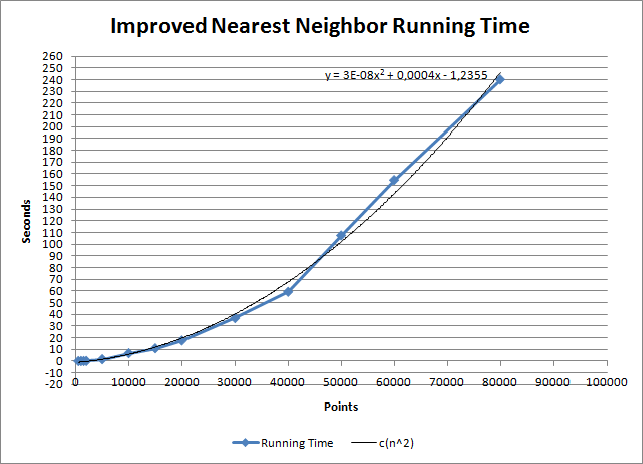
\includegraphics[scale = 0.7]{3ImprovedNearestNeighbor/innRuntimeGraph.png}\\
            Figure 4.2: Graph of \textit{ImprovedNearestNeighbor}'s Running Time
            \label{fig:inn_runnningtime}
          \end{center}

      \noindent The results of the running time are what we expected, again it looks like the algorithm is $O(n^2)$, especially when we introduce the $n^2$ trend line. It may not be that obvious as it was the case with \textit{NearestNeighbor} and \textit{DirectedNearestNeighbor} but we still can conclude using the graph that \textit{ImprovedNearestNeighbor} is $O(n^2)$.
      If we compare the algorithm to \textit{NearestNeighbor} and \textit{DirectedNearestNeighbor}, we see that is slower than \textit{NearestNeighbor}, which is obvious of course since it uses \textit{NearestNeighbor} with an extra function, and faster than \textit{DirectedNearestNeighbor}.\\

    \subsection{Correct output}
    There were a couple of things that went better with \textit{ImprovedNearestNeighbor} than with \textit{NearestNeighbor}. For example the heart of 128 points (See figure HEART 128 vergelijking), which went completely right. Another thing that works much better in Improved Nearest is the following closed curve, when we draw a normal circle with one point at the outside \textit{NearestNeighbor} would fail but the new \textit{ImprovedNearestNeighbor} does not. This is because of the new functionality to insert points at the end, which checks for multiple things which would not be correct if they occur. The fact that the reconstruction of this type of curve has improved is good, since a similar type of curve can be found in several other test-cases we ran.
    See Figure 4.3 to see an example.\\

          \begin{center}
            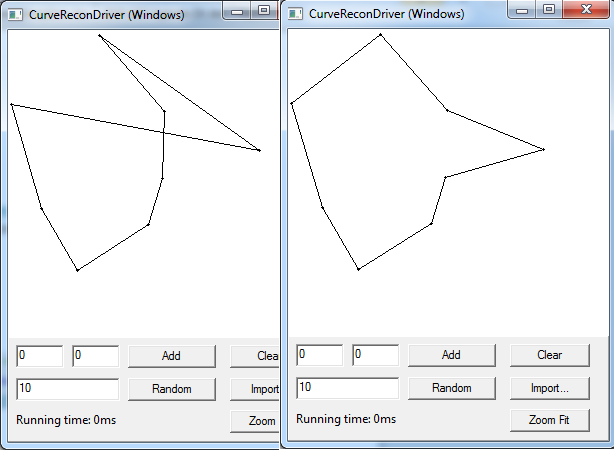
\includegraphics[scale = 0.7]{3ImprovedNearestNeighbor/innPointCirkel.png}\\
            Figure 4.3: Left: Nearest Neighbor Algorithm. Right: Improved Nearest Neighbor Algorithm
            \label{fig:inn_pointcircle}
          \end{center}

   \noindent For example one of the test cases which contains this problem; the Heart with 128 points:\\

          \begin{center}
            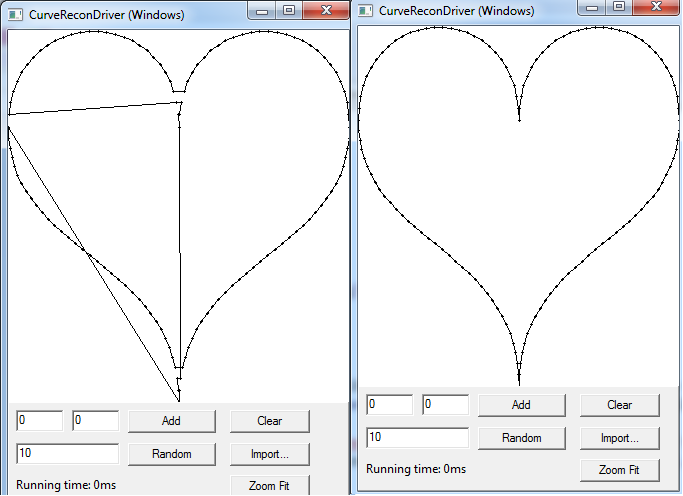
\includegraphics[scale = 0.7]{3ImprovedNearestNeighbor/innHeart.png}\\
            Figure 4.4: Left: Nearest Neighbor Algorithm. Right: Improved Nearest Neighbor Algorithm
            \label{fig:inn_pointcircle}
          \end{center}

    \noindent A test case that still went wrong is the spiral: \\

          \begin{center}
            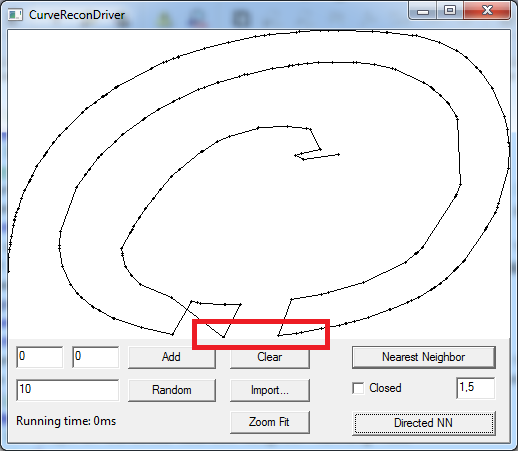
\includegraphics[scale = 0.7]{3ImprovedNearestNeighbor/innSpiral.png}\\
            Figure 4.5: Incorrect Spiral
            \label{fig:inn_pointcircle}
          \end{center}

  \noindent This test case results in the same incorrect reconstruction as with the Nearest Neighbor algorithm. So in this test case the function that inserts lost points at the end didn't have any effect. A suggestion to improve this result would be to add the technic of the Direct Nearest Neighbor to this algorithm. This could result in a much better result.

  \noindent Another test case that went wrong is the Flat with 88 points:\\

            \begin{center}
            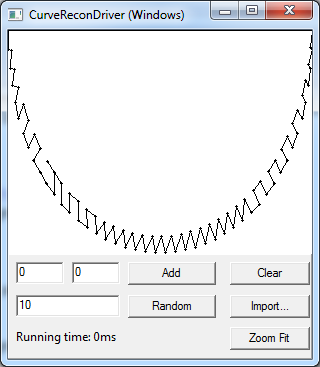
\includegraphics[scale = 0.7]{3ImprovedNearestNeighbor/innFlat.png}\\
            Figure 4.6: Incorrect Flat
            \label{fig:inn_pointcircle}
          \end{center}

  \noindent In this test case we notice some zigzagging, although this is a pretty hard test case since there are only 88 points, the same solution as mentioned above could provide a better reconstruction. Because this test case could probably benefit a lot by checking in which direction the curve is going.

   \subsection{Conclusion}
   We can conclude from the above experiments that Improved Nearest Neighbor really improves a number of problems we first had with the standard Nearest Neighbor algorithm. Especially the function that inserts lost points at the end really provides better results. But still there are a number of test cases that went wrong, to make this number of failing test cases smaller, a combination of the Improved and Directed Nearest Neighbor could maybe be a solution. This could, for example, result in a better reconstruction of the Spiral test case. Another thing that could probably make the reconstructions better is a check for intersections. Since a number of test cases contained a number of intersections which shouldn't be there. For example see the Spiral test case.
   These two suggestions would probably make the Improved Nearest Neighbor even better.
